% This is LLNCS.DEM the demonstration file of
% the LaTeX macro package from Springer-Verlag
% for Lecture Notes in Computer Science,
% version 2.4 for LaTeX2e as of 16. April 2010
%
\documentclass{llncs}
\usepackage{graphicx}
\usepackage{wrapfig}
\usepackage{makeidx}  % allows for indexgeneration
\usepackage{bibspacing}
\usepackage{fancyvrb}
\setlength{\bibspacing}{\baselineskip}
\usepackage[tight,footnotesize]{subfigure}

\newcommand{\mySection}[1]{\vspace{-5pt}\section{\hskip -1em.~~#1}\vspace{-10pt}}
\newcommand{\mySubSection}[1]{\vspace{-5pt}\subsection{\hskip -1em.~~#1}\vspace{-10pt}}
\newcommand{\mySubSubSection}[1]{\vspace{-5pt}\subsubsection{\hskip -1em.~~#1}\vspace{-5pt}}
\newcommand{\tableref}[1]{Table~\ref{tab:#1}}
\newcommand{\figref}[1]{Fig.~\ref{fig:#1}}
\newcommand{\Hao}[1]{$\clubsuit$\footnote{HAO: #1}}

%\setlength{\textheight}{22cm}
%\setlength{\textwidth}{12cm}
%%%\setlength{\columnsep}{0.2in}
%%%\setlength{\botmargin}{-1.0in}
%%\setlength{\headheight}{+0.5in}
%\setlength{\headsep}{-0.2in}
%%\setlength{\parindent}{1pc}
%\setlength{\oddsidemargin}{+.4in}
%\setlength{\evensidemargin}{+.4in}

\begin{document}
%
\frontmatter          % for the preliminaries
%
\pagestyle{headings}  % switches on printing of running heads
%\addtocmark{Hamiltonian Mechanics} % additional mark in the TOC
%
          % start of the contributions
%
\title{A High-Level Behavior Language for Electro-Physiology Heart Modeling}
%\titlerunning{Pacemaker Verification}  % abbreviated title (for running head)
%\author{Zhihao Jiang,  and Rahul Mangharam}\vspace{-10pt}
\authorrunning{Jiang et al.} % abbreviated author list (for running head)
%\institute{University of Pennsylvania, Philadelphia PA, USA}

\maketitle              % typeset the title of the contribution
\vspace{-10pt}


% \begin{figure*}
% \centering

% 		\subfigure {
% 				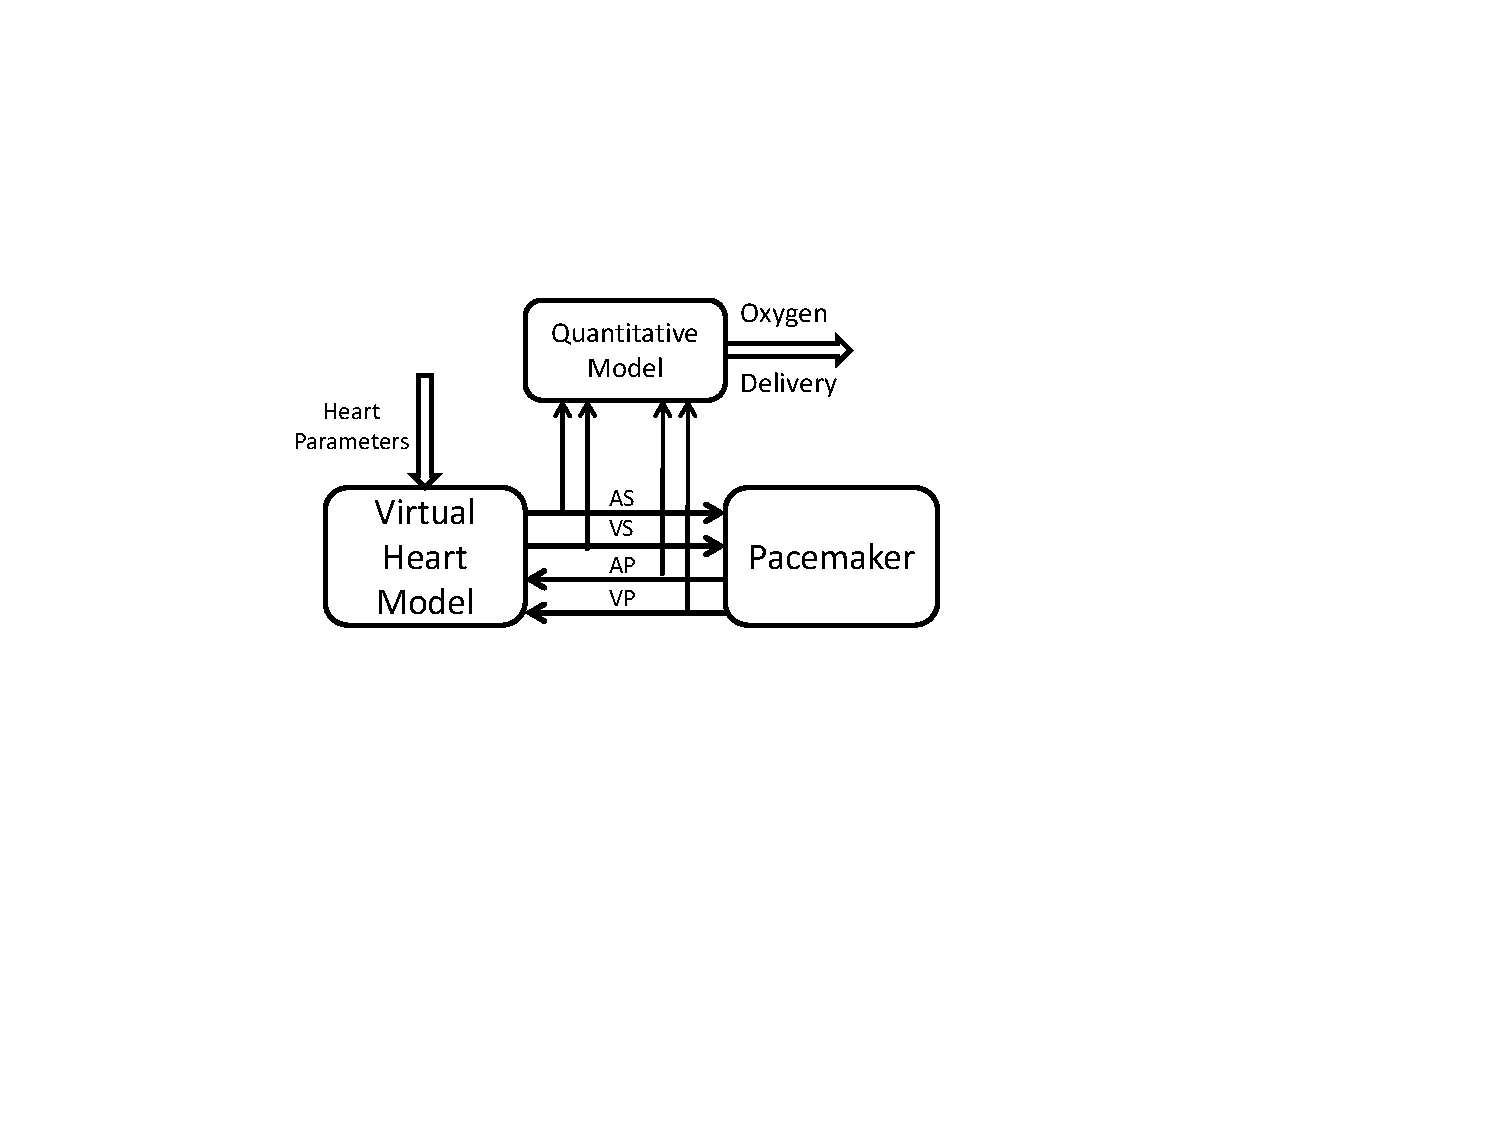
\includegraphics[width=0.45\textwidth]{figs/overall.pdf}
% 				\label{fig:overall}
% 		} 
% 		\subfigure {	
% 			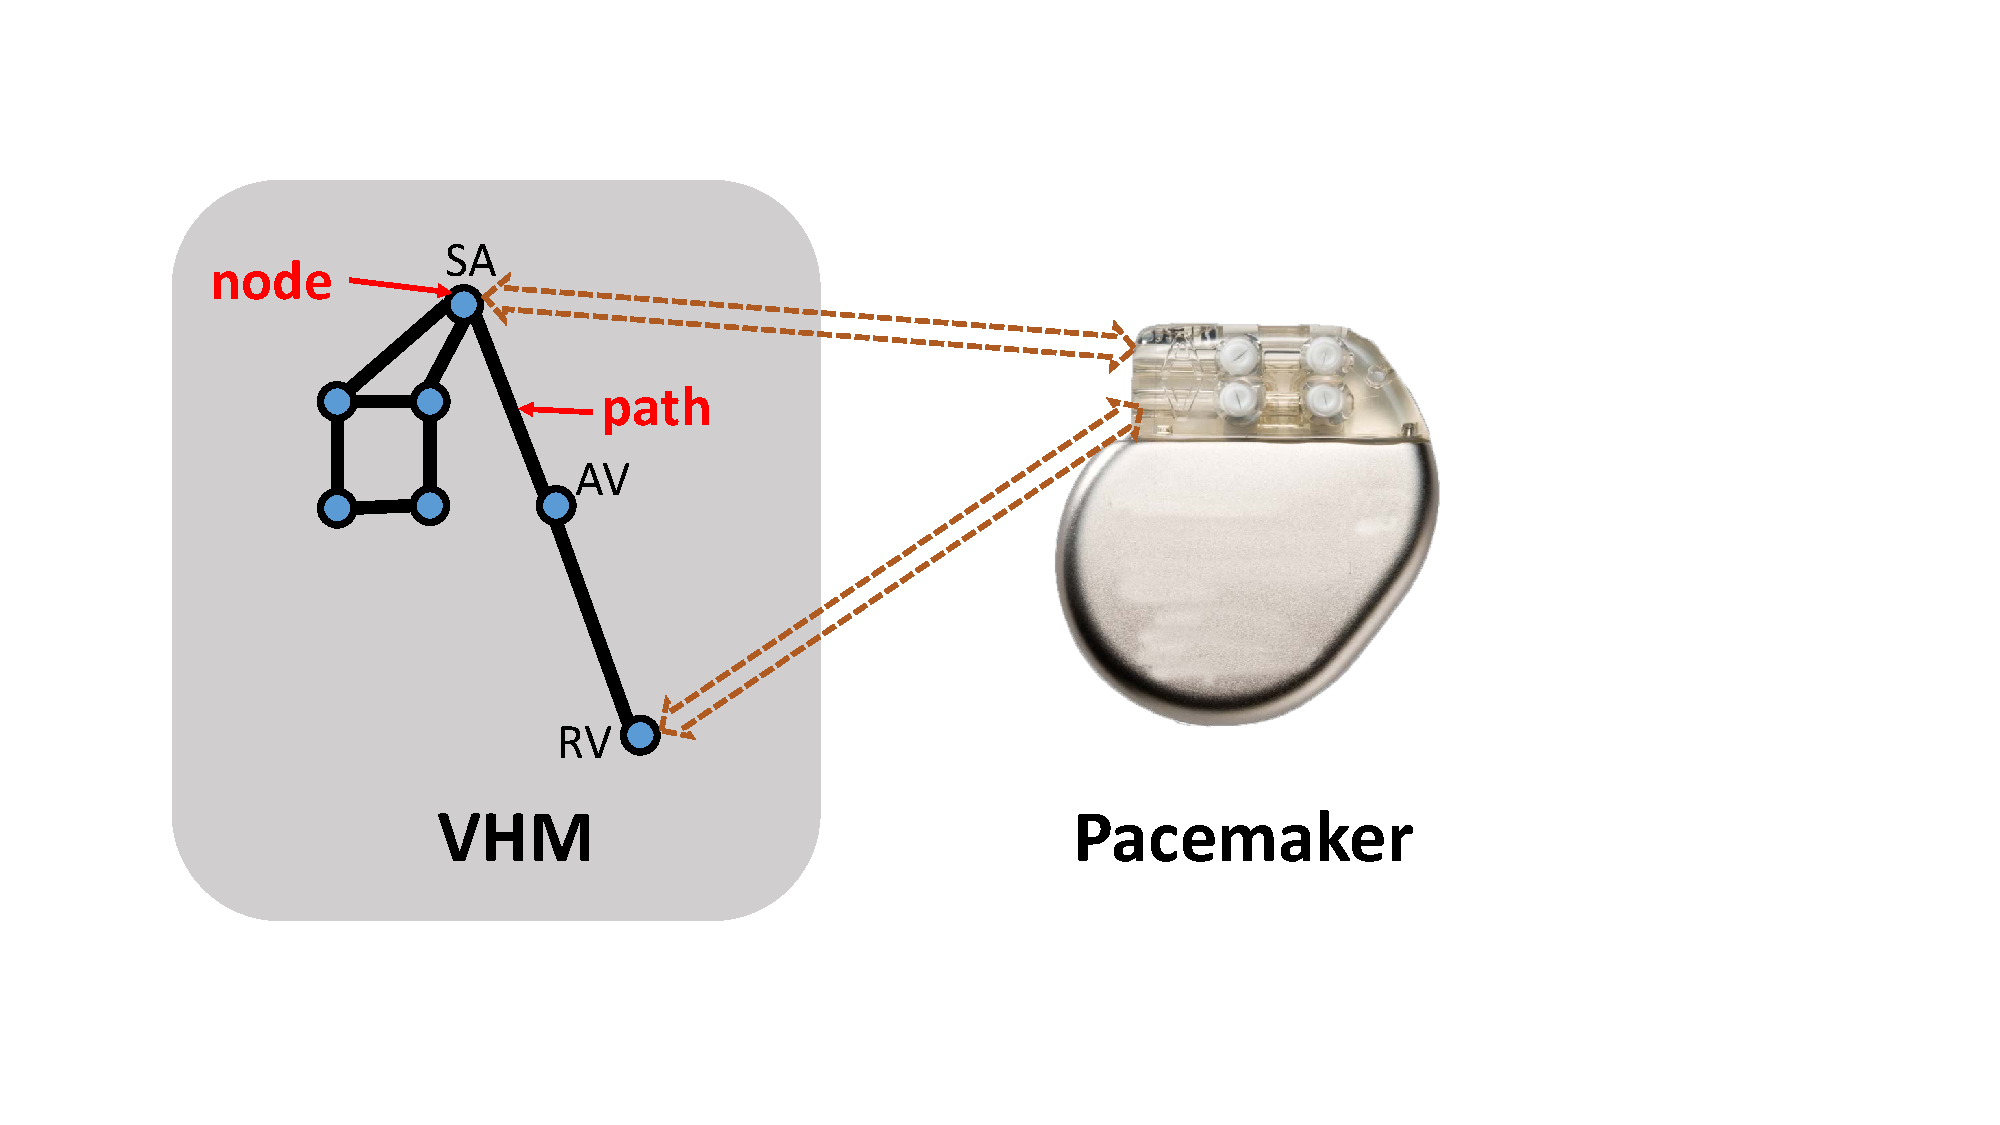
\includegraphics[width=0.45\textwidth]{figs/layout.pdf}
% 			\label{fig:VHM}
% 		}
        
%         	\caption{(a) System layout. (b) A sample closed-loop system}
% \end{figure*}
\section{Introduction}

Generally, a model is used to solve a problem. The best model then is the one that solves your problem with minimum complexity (including time complexity).

Simply using a model with great detail can be detrimental to solving the problem.

Thus, in dynamic systems, it is best for the model to embody the necessary set of behaviors (and no more). 

But, how do you know you have the detail included in your model such that the behaviors of interest are properly captured to solve your problem?

*a tree*
\subsection{Problem Statement}
\begin{itemize}
	\item If system tuned using environment models doesn't work on real environment, nobody knows why. (Model/tool developer vs. application engineers, different domain expertise)
    \item Assumptions/approximations made during the model development are not well-documented (fundamental problem of MBD)
    \item So many models available at different abstraction level, which one to chose? What is the most appropriate level of abstraction? How to validate the model?
    \item Model validation should not be only judged by how realistic the model is
    \item Used CEGAR for model selection, analyzing the execution requires reasoning which relies on domain knowledge 
\end{itemize}
We use pacemaker as case study to demonstrate
\begin{enumerate}
	\item A behavior layer between the requirements and the model structure: better linking requirement with the model structure, reasoning refinement/requirements at behavior level instead of model structure level. 
    \item A rule-based environment model abstraction flow: Easier to validate, also provide traceability on the effects of abstraction on model behaviors
    \item We use the behavior layer to describe closed-loop requirements
    \item We use the behavior layer to choose the appropriate heart abstraction according to the constraints in the requirements, thus automating the model refinement in \cite{STTT13}
\end{enumerate}
\begin{figure}[!t]
		\centering
		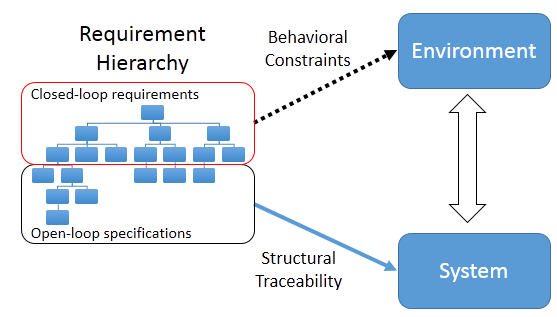
\includegraphics[width=0.7\textwidth]{figs/requirement.png}
		%\vspace{-5pt}
		\caption{\small Stroke Volume as a function of heart rate and AV interval}
		  %\vspace{-15pt}
		\label{fig:req}
\end{figure}
\subsection{Requirement Engineering}
The requirements for the software are initially \textbf{closed-loop requirements} which describe the high-level closed-loop behaviors of the system and the environment. For example an autonomous car will have a requirement of "no collision with pedestrians", which can be interpreted into a closed-loop behavioral requirement: "the car and the pedestrian should not be in the same location at the same time". The closed-loop requirements are then brokend down into executable lower-level open-loop requirements, or specifications that are explicit descriptions of how the system can achieve the closed-loop requirements. In requirement engineering, \emph{traceability} from system design to open-loop specifications, as well as from open-loop specifications to closed-loop requirements are maintained through documentation. 
\begin{itemize}
	\item The link between requirement and environment missing
    \item link mostly through behaviors
\end{itemize}
\subsection{Model Abstraction}
\begin{itemize}
	\item Observable state space don't change
    \item Each abstraction is a mapping from internal state space to observable state space
    \item More abstracted model has less \textbf{resolution} on the observable state space 
    \item More refined model can describe
\end{itemize}
\begin{figure}[!t]
		\centering
		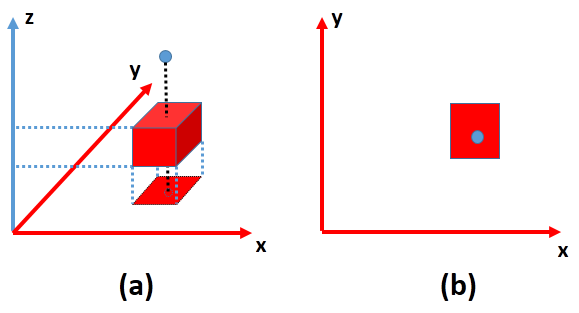
\includegraphics[width=0.6\textwidth]{figs/mapping.png}
		%\vspace{-5pt}
		\caption{\small Stroke Volume as a function of heart rate and AV interval}
		  %\vspace{-15pt}
		\label{fig:map}
\end{figure}
\subsection{Closed-loop Evaluation of Medical Device Software}
\begin{itemize}
	\item Why closed-loop?
    \item Different level of abstraction for the environment model
    \item CEGAR
\end{itemize}
\subsection{Difference With CEGAR in terms of finding the right level of abstraction}
Assume an environment model (Model 1) has 3 state variables \textsf{x,y,z} but only \textsf{x,y} are observable. The state space of the model is shown in \figref{map}.(a). The error states are represented with the red cube. An abstraction has been made to reduce the state space to just \textsf{x} and \textsf{y} axis (Model 2). The error stats are also mapped onto the 2D plane.  
\begin{itemize}
	\item Due to observability, there can be multiple internal environmental behaviors that can result in the same observable trace. When an observable execution trace is returned as a counter-example, This ambiguity is mostly introduced during model abstraction and cannot be distinguished using CEGAR
    \item CEGAR refine the model during closed-loop evaluation. Our approach can refine the model as early as the requirements are specified
    
\end{itemize}
\section{Behavior Layer for Model-based Design}
*Analogy of traffic control*
\subsection{High-level EP Heart Behaviors}
The observable EP heart behaviors are local depolarizations that can be recorded by placing electrodes against the inner heart wall. With these recordings, the physicians developed their own perspective of describing heart behaviors in terms of generation and conduction of depolarizations throughout the heart. The pacemaker has only two leads into the heart, thus offering only two observable points for local depolarizations.


The following are the most fundamental behaviors to describe the behavior of the heart.
\begin{itemize}
	\item Self-activation (self):increase the number of activations
    \item Conduction (cond): maintain the number of activations \Hao{Need to work on detail of this}
    \item Refractory Blocking (block): reduce the number of activations
    \item External Pacing (pace): increase the number of activations

\end{itemize}


We name the behavior of depolarization of certain heart tissue \emph{activation (act)}. It can be triggered by both \emph{self-activation} and \emph{conduction}. Ideally one activation generated either by self-activation or pacing will activate all the activatable tissue in the heart \textbf{once}.
\begin{figure}[!t]
		\centering
		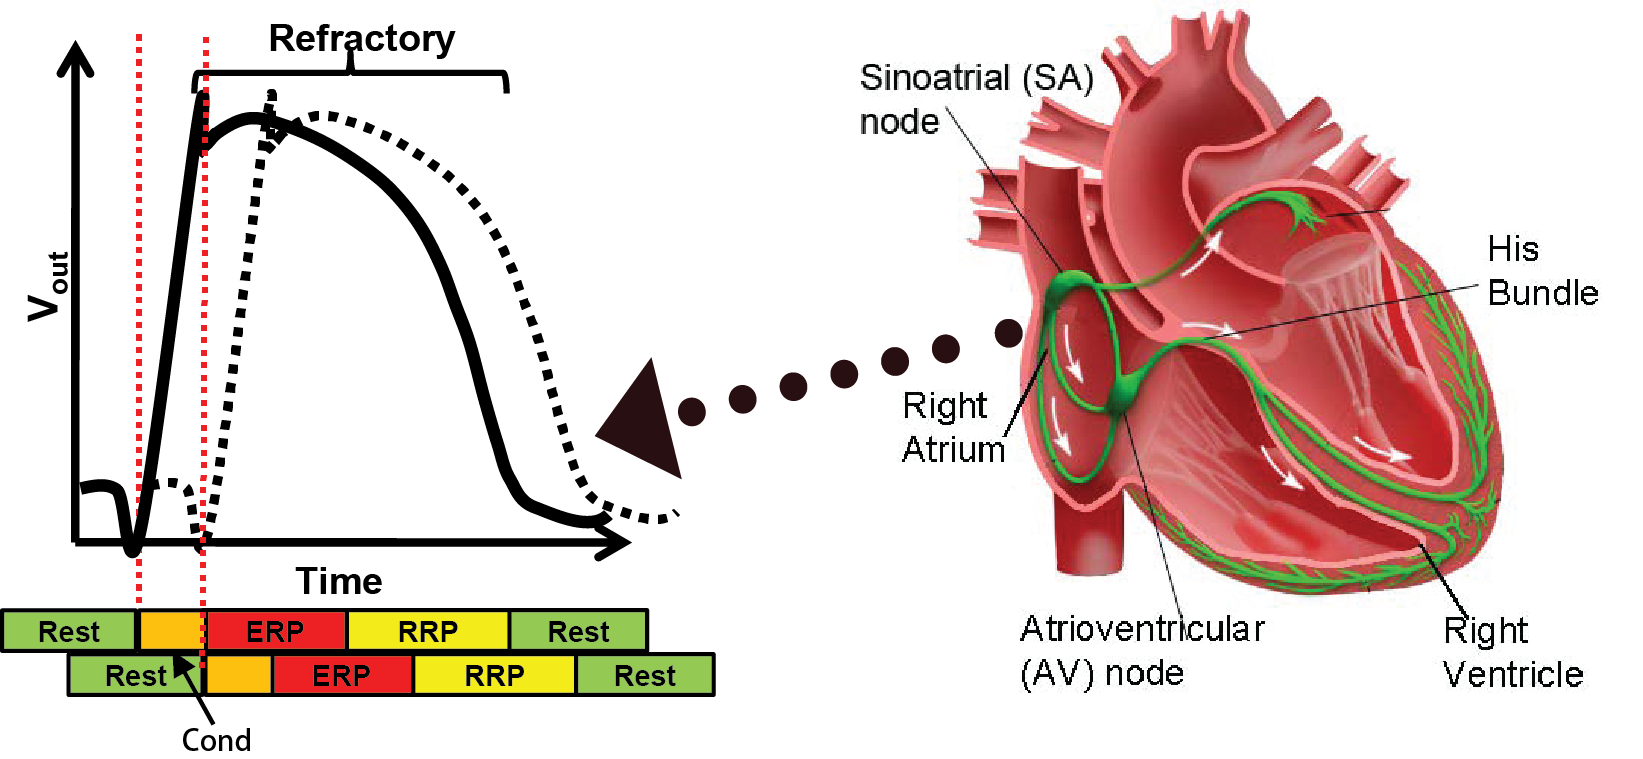
\includegraphics[width=0.8\textwidth]{figs/basic.png}
		%\vspace{-5pt}
		\caption{\small Stroke Volume as a function of heart rate and AV interval}
		  %\vspace{-15pt}
		\label{fig:SV}
\end{figure}

First there are identified structures within the electrical conduction system of the heart. Without forming a circle in the heart, the self-depolarization always happens in the \emph{SA node ($SA$)}. After depolarizing the whole atria, the depolarization signal reaches the \emph{AV node ($AV$)}. Then the signal travels through the \emph{His Bundle (His)} and depolarize the whole ventricle, including the \emph{Right Ventricular Apex (RVA)} through the \emph{Pukinje Fibers (Puk)}. 

Let $S$ be the set of structures and $B$ be the set of behaviors. We represent the behavior associated with a structure $s\in S$ using $s.b$. 

So we have the following behaviors: \textsf{SA.self}, \textsf{SA.block},  \textsf{SA\_AV.cond}, \textsf{AV.block}, \textsf{His.cond}, \textsf{His.block}, \textsf{Puk.cond}, \textsf{Puk.block}, \textsf{RVA.block}. Some tissue in the left atrium and the ventricles can self-depolarize prematurely. They are called \emph{Premature Atrial Contraction (PAC)} and \emph{Premature Ventricular Contraction (PVC)} respectively. So we have two more behavior: \textsf{PAC.self} and \textsf{PVC.self}. A typical heart cycle can be represented by a sequence of behaviors: \textsf{SA.self$\rightarrow$SA\_AV.cond $\rightarrow$ His.cond$\rightarrow$Puk.cond$\rightarrow$Vent.act}

\subsection{Behavior Abstraction}
\Hao{Need formal description}Happens along with structural abstraction.
\begin{itemize}
	\item Renaming: sometimes behaviors are assigned to another structure and their old names no longer make sense. Or we can say that Renaming is a special case for Inclusion
    \item Inclusion: can also be used for constructing higher-level behaviors. e.g. \textsf{Atrial.self=\{SA.self,PAC.self\}}
    \item Remove: Behaviors like Block can be removed without \textbf{reducing} the observable behaviors
\end{itemize}
\subsection{Behavior Abstraction Criteria}
There are criteria that have to be followed when abstracting behaviors. These criteria are based on domain knowledge.
\begin{enumerate}
	\item When a \textsf{block} behavior can be safely removed
    \item How to combine \textsf{self-cond-self} with one \textsf{self}
\end{enumerate}
\subsection{High-level behaviors of the heart}
We can use the behaviors to construct high-level behaviors of the heart to represent different heart conditions.\\
Intrinsic atrial activations:\\
\textsf{Atrial.self=\{SA.self,PAC.self\}}\\
Intrinsic Ventricular activations:\\
\textsf{Vent.self=\{PVC.self\}}

\section{Rule-based Heart Model Abstraction}
In STTT, the heart model abstractions were directly given and their timed-simulation relationship are proved with text explanation. State graphs had to be given to show behavior abstraction, which is not effective and no-one will ever read and convinced the validity of the model. With the rule-based heart model, we can validate the initial model and all the rules applied to the model. The abstraction rules not only change the structure of the model, but also the behaviors. The structural changes for these abstractions can be found in \cite{STTT}. Here we show the behavior changes during these abstractions.
\subsection{Abstraction Intuition}
Abstract both the structure and internal behaviors without reducing the \textbf{observable behaviors}. So the definition of refinement is to add essential internal behaviors back to the model to represent more specific environmental conditions.
\begin{figure}[!t]
		\centering
		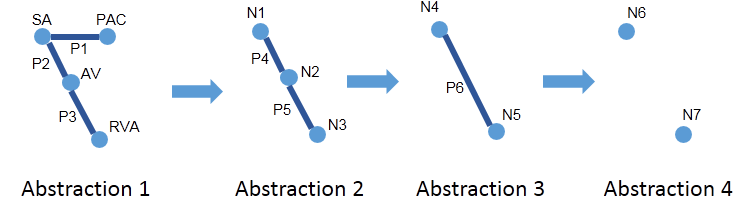
\includegraphics[width=0.9\textwidth]{figs/abs.png}
		%\vspace{-5pt}
		\caption{\small Stroke Volume as a function of heart rate and AV interval}
		  %\vspace{-15pt}
		\label{fig:SV}
\end{figure}
\subsection{Abstraction 1: HM1}
\textsf{SA.self=\{SA.self\}\\
PAC.self=\{PAC.self\}\\
AV.block=\{AV.block\}\\
P2.cond=\{SA\_AV.cond\}\\
P3.cond=\{His.cond\}\\ 
RVA.act=\{PVC.self,P3.cond\}}
\subsection{Abstraction 2: HM2}
\textsf{N1.self=\{SA.self,PAC.self\}\\
N2.block=\{AV.block\}\\
P4.cond=\{P2.cond\}\\
P5.cond=\{P3.cond\}\\
N3.act=\{RVA.act\}}
\subsection{Abstraction 3: HM3}
\textsf{N4.self=\{N1.self\}\\
N5.self=\{N4.self\}\\
P6.cond=\{P4.cond,P5.cond\}\\
P6.block=\{N2.block\}}
\subsection{Abstraction 4: HM4}
\textsf{N6.self=\{N3.self,P6.cond\}\\
N7.self=\{N5.self,P6.cond\}}
\section{Case Study: Automated Requirement-based Heart Model Selection}
\subsection{Annotating requirements with behavior objects}
Closed-loop requirements are mostly \textbf{conditional}, meaning that it should hold under certain environmental condition. For example, the following requirement:\\
\textsf{R1: When the intrinsic activation in the atria and ventricles are both less than 100bpm, the ventricular rate is less than 100bpm}\\
The requirement constrains on the \textsf{Atrial.self} and \textsf{Vent.self}, and reason about \textsf{Vent.act}


\subsection{Rules for Heart Model Eligibility Check}

\begin{itemize}
	\item The behavior (or its renames) constrained in the condition of the requirement should not be abstracted with other behaviors in the heart model
    \item 
    
\end{itemize}

\begin{Verbatim}
function [status,message]=eligible(HM,Req)
	for all BehaveObj1 in Req.condition
    	for all the BehaveObj2 in HM.behavior
        	while (BehaveObj1 not in BehaveObj2)||(BehaveObj2 not rename of BehaveObj1)
            	if 
\end{Verbatim}

\subsection{Example}
We perform \textsf{eligible(HM4,R1)} and the check fails, since \textsf{Atrial.self=N1.self=N4.self$\in$N6.self}. The check also suggest that \textsf{N3.self} and \textsf{P6.cond} should be seperated. If we go to HM3 and \textsf{eligible(HM3,R1)} is successful. So HM3 is the suggested heart model for requirement \textsf{R1}.
% \begin{figure}[!h]
% 		\centering
% 		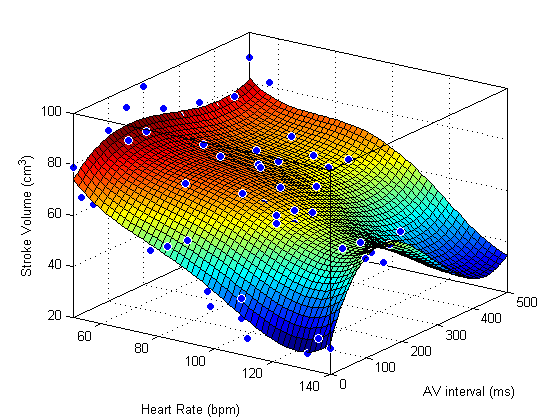
\includegraphics[width=0.4\textwidth]{figs/SV.png}
% 		%\vspace{-5pt}
% 		\caption{\small Stroke Volume as a function of heart rate and AV interval}
% 		  %\vspace{-15pt}
% 		\label{fig:SV}
% \end{figure}


% ---- Bibliography ----
%
\bibliographystyle{unsrt}
{ \small 
\bibliography{bibliography}
}
\end{document}